\documentclass[12pt]{article}
\usepackage{epsfig}
\usepackage{graphicx}
\usepackage{color}
\usepackage[frenchb]{babel}
\usepackage{subfigure}
\usepackage{algorithm}
\usepackage{algpseudocode}
\usepackage{amsmath}
\usepackage{url}
\usepackage{listings}


% Pour pouvoir utiliser les accents directement dans LaTeX, sans utiliser les commandes \'
%\usepackage[latin1]{inputenc} % entree 8 bits iso-latin1
\usepackage[utf8]{inputenc} % entree 8 bits utf8, fonctionne avec MikTeX sur Windows.
\usepackage[T1]{fontenc}      % encodage 8 bits des fontes utilisees

% Pour agrandir les marges
\addtolength{\oddsidemargin}{-.875in}
\addtolength{\evensidemargin}{-.875in}
\addtolength{\textwidth}{1.75in}
\addtolength{\topmargin}{-.875in}
\addtolength{\textheight}{1.75in}

\makeatletter\renewcommand{\ALG@name}{Algorithme}


\begin{document}
%\selectlanguage{frenchb}
\title{GLO-4001/GLO-7021 Introduction à la robotique mobile \\  TP1 Version complète 1.0 \\ Date de remise : 23 octobre 2017 à 23h55}
\author{En équipe de 1 à 2.}
\maketitle


{\bf Attention! N'oubliez pas d'attacher le code de toutes les questions dans la remise .zip de votre travail. Si les codes sont manquants, nous pourrons retirer jusqu'à 20\% de la note. }

Pour tous les étudiants, vous devez fournir un rapport en un seul document (format pdf) et les fichiers matlab ou Python zippé. Pour toutes les questions, n'oubliez pas de mettre le détail des calculs.

Pour les étudiants en GLO-7021, veuillez noter qu'une présentation déficiente dans le rapport (manque de clarté, orthographe et grammaire, police de caractère illisible sur figure matlab, etc) pourra entraîner une pénalité allant jusqu'à 10 \% de la note. Le rapport doit aussi obligatoirement être formaté avec Latex.


% ================== Carte =======================
\section{Carte 2D à partir d'un gyroscope et d'un capteur de distance (15 pts)}

\subsection{Carte 2D locale (5 pts)}
\label{CarteLocale}

\subsubsection{Calculs}
Pour pouvoir créer un nuage de point sur un plan 2D, il faut utiliser nos données pour obtenir une variété de points x, y.
Pour cela, il faut:
\begin{enumerate}
        \item Convertir la tension de notre capteur en distance.
        \item Convertir la vitesse angulaire du gyroscope en angle.
        \item Obtenir un point (x, y) avec la distance et l'angle.
\end{enumerate}

\textbf{Convertir la tension du capteur}
Soit la fonction du capteur avant bruit:
\[ z(d) = 1/d \]

Comme le capteur est bruité, il faut consid\'erer celui-ci. On mod\'elise donc la fonction avec une gaussienne:

\textbf{Convertir la vitesse angulaire}
Soit :
\[ \frac{d\theta}{dt} = g \] o\'u g est la vitesse angulaire.
On peut approximer cela \`a:
\[ \frac{\Delta \theta}{\Delta t}  = g\]
Avec le temps t noté, on peut trouver la valeur de $\theta$ en ajoutant $\Delta t * g $ ou $ (t_{valeur précédente} - t_{valeur courante}) * g$.

Toutefois, cette technique va cumuler de l'erreur avec le temps.
Pour Réduire l'erreur du à l'intégration:

\textbf{Obtenir un point (x, y)}

Soit avec la trigonométrie:
\[ x = d*\cos(\theta) \] \[ y = d*\sin(\theta) \]

\subsubsection{Code}
Le fichier question1.py contient le code utilisé pour former la carte 2D.
\subsubsection{Carte}

\begin{figure}[ht]
 \begin{center}
  \begin{tabular}{c}
    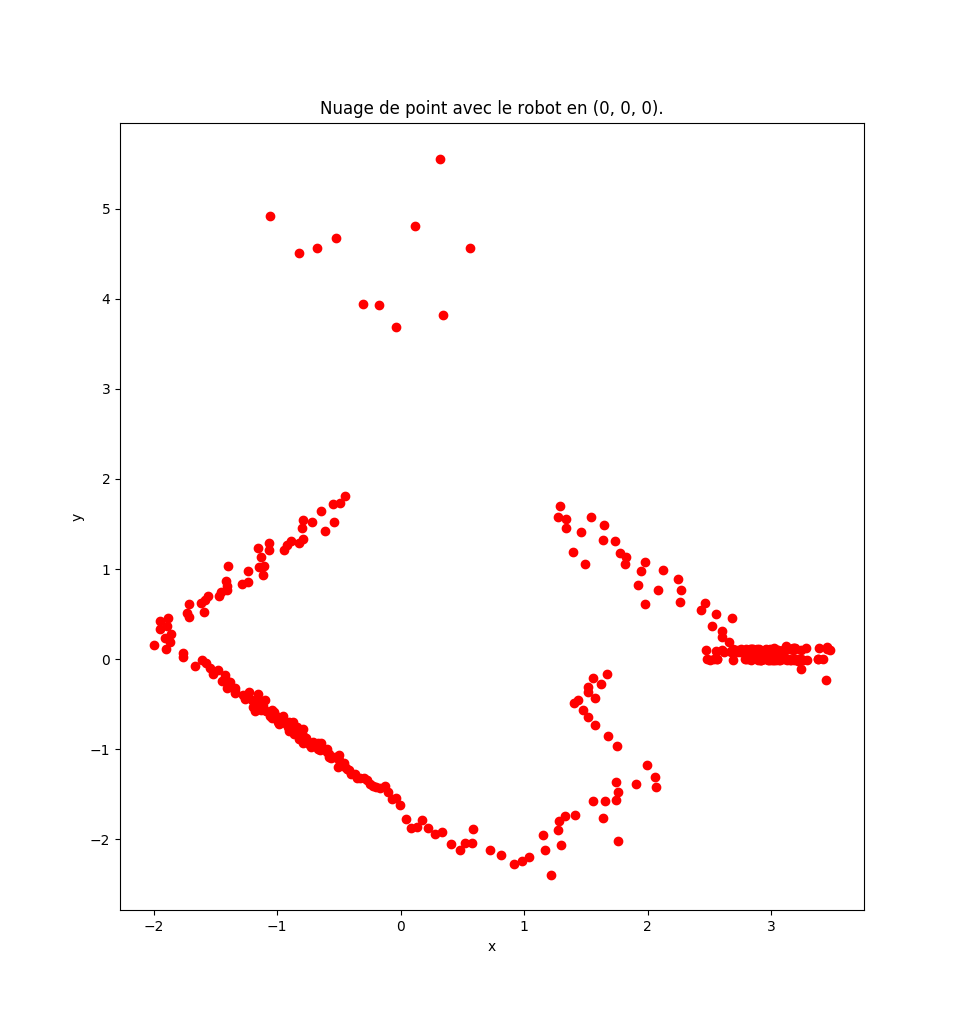
\includegraphics[width=0.75\textwidth]{q1-carte-local.png}
  \end{tabular}
 \end{center}
\vspace{-0.25in}
 \caption{Carte 2D générée avec les données matlab et le code python.}
    \label{carte-2d-locale}
\end{figure}

La figure \ref{carte-2d-locale} représente le nuage de point.

\newpage
\subsection{Localisation du robot dans la carte globale (10 pts)}

\subsubsection{Calculs}
\textbf{Création de $P_{Homogene}$:}

\[ \text{Soit } P_{Homogene} =
\begin{bmatrix}
    x_1 & x_2 & x_3 & ... & x_n \\
    y_1 & y_2 & y_3 & ... & y_n \\
    1   & 1   & 1   & ... & 1   \\
\end{bmatrix}
\]

\textbf{D\'etermination des matrices de transformation T:}

Soit pour faire une translation $[T_x, T_y]$, il faut multiplier $P_{Homogene}$ par la matrice

\[
    T =
    \begin{bmatrix}
        1 & 0 & T_{x} \\
        0 & 1 & T_{y} \\
        0 & 0 & 1
    \end{bmatrix}
    \]

\textbf{D\'etermination des matrices de transformation R:}

Soit pour faire une rotation de $\theta rad$, cela \'equivaut \`a multiplier par la matrice
\[
    R =
    \begin{bmatrix}
        \cos{\theta} & -\sin{\theta} & 0 \\
        \sin{\theta} & \cos{\theta} & 0 \\
        0 & 0 & 1 \\
    \end{bmatrix}
    \]

\subsubsection{Code}


\subsubsection{Réponse}

% ================== CAMERA =======================
\newpage
\section{Modèle de caméra et positionnement par caméra}

\subsection{Génération d'une image (5 pts)}
\label{generation_image}
\subsubsection{Calculs}
Soit la relation entre le point correspondant [u, v] et la position dans le monde r\'eel $ [L_{ix}, L_{iy}, L_{iz}] $
\[ \left[ {\begin{array}{c}
                u \\
    v \\ \end{array} } \right] =
    \frac{f}{L_{iz}}
    \left[ {\begin{array}{c} L_{ix} \\ L_{iy} \\ \end{array}} \right]
\]

Comme la valeur $L_y$ est nulle, nous obtenons:


\[ \left[ {\begin{array}{c}
                u \\
    v \\ \end{array} } \right] =
    \frac{f}{L_{iz}}
    \left[ {\begin{array}{c} L_{ix} \\ 0 \\ \end{array}} \right]
=
    \left[ {\begin{array}{c} \frac{f}{L_{iz}} * L_{ix} \\ \frac{f}{L_{iz}} * 0 \\ \end{array}} \right]
=
    \left[ {\begin{array}{c} \frac{f}{L_{iz}} * L_{ix} \\ 0 \\ \end{array}} \right]

\]

On peut ainsi en conclure que:
\[
    u =  \frac{f}{L_{iz}} * L_{ix}
\]
\[
    v = 0
\]
o\`u u et v sont en pixels, et f = 1200 pixels.

\subsubsection{Code}

Le fichier HelpMePleaseImStuckInAMethodName.py contient la fonction pour convertir la position de $L_i$ en une position d'écran [u, v].

\subsection{Estimation de la pose de la caméra à partir des angles $\alpha$ et $\beta$ (5 pts)}
\subsubsection{Calculs}
\subsubsection{Code}
\subsubsection{Réponse}

\subsection{Impact du bruit sur l'estimation des repères (10 pts)}
\subsubsection{Calculs}
\subsubsection{Code}
\subsubsection{Réponse}

% ================== STEREO =======================
\newpage
\section{Imagerie stéréo  (15 pts)}

\subsection{Distance focale $f$ (4 pts)}
\subsubsection{Calculs}
Pour obtenir f, il faut connaître les valeurs [u, v] de la tour verte.
Mesur\'ee avec une r\`egle, on obtient:
\[ u = 0 px \text{(centre de l'image)}\]
\[ v = 310 px\]
Sachant que:
\[ \text{Axe des v: } 0.7cm = 200px \]
En reprenant la fonction trouv\'ee en \ref{generation_image}, on sait que :

\[
    u =  \frac{f}{L_{iz}} * L_{ix}
\]
\[
    v =  \frac{f}{L_{iz}} * L_{iy}
\]
On isole $f$ dans l'\'equation de v:
\[
    f =  \frac{v * L_{iz}}{L_{iy}}
\]

Comme on sait que la tour fait 15cm de hauteur ($L_{iy} = 15$) et que celle-ci est \`a une distance de 95cm de la cam\'era ($L_{iz} = 95$):
\[
    f =  \frac{v * L_{iz}}{L_{iy}} = \frac{310px * 95 cm}{15cm} = 1963.33 px = 2000 px
\]


\subsubsection{Code}
\subsubsection{Réponse}
La distance focale est d'environ 2000 pixels.

\subsection{Estimation de la distance $A_z$ de chaque tour LEGO (6 pts)}
\label{estimation_distance_Az}
\subsubsection{Calculs}

\begin{table}[h]
\caption{Disparit\'e $d$ mesur\'ee avec la r\`egle}
\label{TableCoord}
\begin{center}
\begin{tabular}{|c|c|c|c|}
\hline
    tour   &  $u_{gauche}$  &  $u_{droite}$  &  $d$ $(u_g - u_d)$ \\
\hline
    rouge  & --1.75cm & -2.65cm & 0.90cm \\
    bleu   & 1.70cm & 0.50cm & 1.20cm \\
    jaune  & 2.50cm & 1.65cm & 0.85cm \\
\hline
\end{tabular}
\end{center}
\end{table}

Pour convertir la disparit\'e en pixels, on utilise la r\`egle de de trois sachant que:

\[ \text{Axe des u:} 1.2cm = 200px \]


\begin{table}[h]
\caption{Disparit\'e $d$ en pixels}
\label{TableCoord}
\begin{center}
\begin{tabular}{|c|c|c|c|}
\hline
    tour   &  $d$ \\
\hline
    rouge  &  150px \\
    bleu   &  200px \\
    jaune  &  140px \\
\hline
\end{tabular}
\end{center}
\end{table}

On peut trouver $A_z$ avec la formule:
\[ A_z = \frac{f \dot b}{d}\]
Avec f = 2000px et b = 5cm.

\subsubsection{Code}
\subsubsection{Réponse}

\begin{table}[h]
\caption{Distance en $z$ des centres des faces des colonnes.}
\label{TableCoord}
\begin{center}
\begin{tabular}{|c|c|}
\hline
 tour   & $A_z$ \\
\hline
 rouge  & 67cm \\
 bleu   & 50cm \\
jaune   & 71cm \\
\hline
\end{tabular}
\end{center}
\end{table}


\subsection{Estimation de la coordonnée $A_x$ de chaque tour LEGO (5 pts)}
\subsubsection{Calculs}
On r\'eutilise les valeurs de $u_{gauche}$ mesur\'ees en \ref{estimation_distance_Az}.
Puis, on les convertie en pixels.

\begin{table}[h]
    \caption{$u_{gauche}$ en pixels}
\label{TableCoord}
\begin{center}
\begin{tabular}{|c|c|}
\hline
    tour   &  $u_{gauche}$\\
\hline
    rouge  & -290px  \\
    bleu   & 280px   \\
    jaune  & 420px   \\
\hline
\end{tabular}
\end{center}
\end{table}

Avec la trigonométrie, on peut conlure que $u_{gauche} \propto A_x$ soit :
\[ u_g = \frac{f}{A_z}A_x\]
\[ A_x = \frac{u_g \dot A_z}{f} \]
Sachant que $f = 2000px$ et en utilisant les valeurs de $A_z$ trouvées en \ref{estimation_distance_Az}.

\subsubsection{Code}
\subsubsection{Réponse}

\begin{table}[h]
\caption{Coordonnée en $x$ des centres des faces des colonnes.}
\label{TableX}
\begin{center}
\begin{tabular}{|c|c|}
\hline
 tour   &  $A_x$ \\
\hline
 rouge  &  -9.7cm     \\
 vert   &  0.0cm  \\
 bleu   &  7.0cm    \\
 jaune  &  15cm     \\
\hline
\end{tabular}
\end{center}
\end{table}


% ==================  FAST =======================
\newpage
\section{Extracteur de coin FAST (13 pts)}
 \label{SectionFAST}

\subsection{Fonction d'extraction des coins FAST (7 pts)}
Codez une fonction d'extraction de coins basée sur la méthode FAST, pour des cercles tels que montré à la Figure~\ref{FastPixelOrder}. Notez que vous cherchez un coin ayant 12 pixels continus sur l'arc qui satisfassent le critère. La fonction a le prototype suivant :
\vspace{-0.22in}
\begin{lstlisting}
[IsFastCorner IntensiteCoin] = DetectionCoinFAST(Image, Centre, Seuil)
\end{lstlisting}
où les arguments en entrée sont :
\begin{itemize}
\item {Image} une image (en noir et blanc);
\item {Centre} un vecteur donnant la coordonnée x-y pour laquelle tester la présence d'un coin dans l'{Image};
\item {Seuil} le seuil $t$, tel que spécifié dans les équations de l'acétate 134 de \texttt{03-VisionII.pdf};
\end{itemize}
et les sorties sont :
\begin{itemize}
\item {IsFastCorner} indique la présence ou l'absence d'un coin (valeur binaire);
\item {IntensiteCoin} donne l'intensité du coin représenté par la somme $V$, telle que spécifiée à l'acétate 135;
%\item \mcode{Orientation} donne l'orientation du coin, en radian, basée sur l'acétate 145.
\end{itemize}

\begin{figure}[ht]
 \begin{center}
  \begin{tabular}{c}
    \includegraphics[width=0.25\textwidth]{FastPixelOrder.png}
  \end{tabular}
 \end{center}
\vspace{-0.25in}
 \caption{Position des pixels à tester pour le détecteur de coin FAST. Les numéros sont à titre indicatif.}
 \label{FastPixelOrder}
\end{figure}

\subsection{Test de votre fonction \texttt{DetectionCoinFAST} sur une image réelle (6 pts)}
Vous allez maintenant tester votre détecteur de coin une image réelle, à partir d'un jeu de données qui a été capturé sur l'île de Devon dans l'arctique canadien par un robot mobile de l'équipe du Prof.
Barfoot (U. Toronto). Cette île est reconnue mondialement pour sa similarité avec le sol martien, et sert donc souvent de lieu d'essai pour la robotique interplanétaire.
L'image en question est \texttt{bw-rectified-left-022146small.png}.
Parcourez toute cette image (sauf la bordure à l'intérieur de 8 pixels\footnote{Car il ne sera pas possible d'extraire les features BRIEF de la question suivante pour les bordures.}) et trouvez tous les coins, avec la valeur de {Seuil} de 10\footnote{Les intensités dans l'image sont entre 0 et 255, car codé en entier non-signé de 8 bits ({uint8})}.
Pour chaque coin trouvé, marquez sa position à l'aide d'un petit cercle rouge (option {`ro'}).
Attention! Dans matlab, la fonction \mcode{imshow} intervertie les axes x-y.
Pour tracez un cercle rouge qui indique qu'un coin se situe autour du pixel \mcode{Image(X,Y)}, vous devez faire :
\vspace{-0.22in}
\begin{lstlisting}
imshow(Image)
hold on
...
plot(Y,X,'ro');
\end{lstlisting}
Combien de coins trouvez-vous dans cette image? Quel pourcentage des pixels sont donc considérés comme des coins? Pourquoi cette scène génère-t-elle ce nombre de coins ? Quelles régions de l'images contiennent plus de coins? Moins de coins?

Incluez aussi dans votre rapport l'image avec les coins trouvés.


%\subsection{Analyse des résultats (GLO-7021 seulement) (5 pts)}
%Afin de limiter le nombre de coin à traiter, il est possible d'utiliser un heuristique simple, qui permet de ne conserver que les coins les plus forts, basé sur la valeur \mcode{IntensiteCoin}. Cependant, pour utiliser un tel heuristique, il est important de comprendre la distribution de ces valeurs. Dans un histogramme, montrez la distribution des intensités, pour les coins trouvés. À quoi ressemble cette distribution?


% ================== Descripteur BRIEF =======================

\newpage
\section{Descripteur BRIEF (17 pts pour GLO-4001, 27 pts pour GLO-7021)}
Le descripteur binaire BRIEF est de plus en plus utilisé pour décrire des points de repères naturels dans des problèmes de localisation par caméra. Cette popularité grandissante est en partie dûe à sa facilité de codage, sa robustesse et sa rapidité de calcul. Dans cette question, vous allez explorer l'utilisation de ces descripteurs BRIEF, extraits autour de coins FAST. Pour vous aider, référez-vous au besoin à l'article original du BRIEF : \url{https://www.robots.ox.ac.uk/~vgg/rg/papers/CalonderLSF10.pdf} .

\subsection{Fonction calculant un descripteur BRIEF (3 pts)}
En matlab ou python, écrivez une fonction \texttt{ExtractBRIEF(ImagePatch,BriefDescriptorConfig)} qui accepte une patch d'image noir et blanc de SxS pixels avec S=15, ainsi qu'une structure de données \texttt{BriefDescriptorConfig}. Cette fonction retourne le descripteur utilisant \texttt{BriefDescriptorConfig}, dans un format de votre choix. Cette fonction ne devrait être que quelques lignes de code. Plus d'information sur \texttt{BriefDescriptorConfig} est disponible à la question suivante.

\subsection{Pipeline d'extraction de features sur une paire d'images réelles (9 pts pour GLO-4001, 11 pts pour GLO-7021)}
L'extraction de features visuels est en général une opération coûteuse du point de vue calcul. Ainsi, il est préférable de ne se concentrer que sur des points intéressants dans les images, les \emph{keypoints}. Dans la section~\ref{SectionFAST}, vous avez justement codé une fonction permettant l'extraction de keypoints. Un pipeline d'extraction ressemble typiquement au diagramme de la Figure~\ref{PipelineExtraction}.

\begin{figure}[ht]
 \begin{center}
  \begin{tabular}{c}
    \includegraphics[width=0.6\textwidth]{PipelineExtraction.png}
  \end{tabular}
 \end{center}
\vspace{-0.25in}
 \caption{Pipeline d'extraction des features, utilisé lors de la recherche de points de repères naturels dans des images.}
 \label{PipelineExtraction}
\end{figure}

Implémentez ce pipeline, en utilisant vos deux fonctions \mcode{DetectionCoinFAST} et \mcode{ExtractBRIEF} pour la première et quatrième étape du pipeline. Pour les étudiants en GLO-4001, la suppression des non-maxima locaux est optionnelle. Pour les GLO-7021, implémenter une version approximative de cette suppression, de votre choix. La sélection des coins sera basée sur la valeur de leur intensité \mcode{IntensiteCoin}: vous ne conserverez que ceux dans le 90ème percentile (autrement dit, les 10~\% les plus forts)\footnote{Une manière facile pour identifier ces coins est de trier la liste des coins selon l'intensité, et de ne conserver que un dixième de cette liste.} . Pour les descripteurs, utilisez \texttt{numberOfBits}=256 bits. Dans ce programme, la structure de données \texttt{BriefDescriptorConfig} qui décrit les \texttt{numberOfBits} paires de pixels pour lesquelles les tests sont faits y est  \underline{initialisée une seule fois}. Pour générer ces paires de pixels (obligatoirement de manière aléatoire), utilisez une distribution uniforme (\texttt{rand()}) sur SxS, avec S=15. Ne vous préoccupez pas des doublons possibles sur ces paires de pixels, pour vous sauver du temps de codage. Assurez-vous que ces paires sont des entiers, via la fonction \texttt{ceil()}. Le descripteur doit être extrait dans une fenêtre centrée sur le coin FAST.


\subsection{Appariement features image gauche-droite (5 pts)}
 Appliquez votre pipeline sur les images suivantes :
 \begin{itemize}
 \item \texttt{bw-rectified-left-022146small.png} et
 \item \texttt{bw-rectified-right-022146small.png},
 \end{itemize}
 disponibles dans le répertoire inclus avec ce TP. Ces images sont issues d'une caméra stéréo. Pour chaque descripteur de l'image de gauche, trouvez le feature dans l'image de droite qui a la plus petite distance de Hamming, donc le plus semblable. Ceci constituera l'appariement. Dans dans votre rapport, mettez une image représentant ces matches. Le fond sera l'image de gauche, et chaque ligne verte reliera le feature de gauche au feature de droite associé, comme dans l'image~\ref{ExempleImageMontrantMatches}. Si vous avez trop de lignes, choisissez-en un nombre raisonnable de manière aléatoire (une centaine) pour affichage.

\begin{figure}[ht]
 \begin{center}
  \begin{tabular}{c}
    \includegraphics[width=0.75\textwidth]{ExempleImageMontrantMatches.png}
  \end{tabular}
 \end{center}
\vspace{-0.25in}
 \caption{Image montrant quelques appariements entre les features de l'image gauche (en fond) vers les features de l'image droite. Notez que j'ai épuré ces matches, afin de ne conserver que de très bons. Vous devriez avoir plus de lignes diagonales dans votre résultat.}
 \label{ExempleImageMontrantMatches}
\end{figure}

\subsection{Amélioration de la qualité des matchs GLO-7021 Seulement (8 pts)}
Vous devriez constater que vous avez beaucoup de faux matches dans l'image. Tentez d'améliorer la qualité de ces matches, en utilisant des stratégies de votre choix. Commentez sur l'amélioration apportée par chacune de vos stratégies.

\end{document}
